\subsection{Manejador de alertas}
\label{manejador-alertas}

Ahora que hemos configurado \gls{term:kapacitor}, contamos con una
infraestructura de monitoreo que permite generar alertas ante anomalías
identificadas por condiciones previamente definidas.

Pero lanzar demasiadas alertas puede provocar una serie de situaciones no
deseadas.

Una de las formas más comunes de enviar notificaciones es a través del uso de
correo electrónico. Pero si se genera una alerta cuando falla la conexión a un
servicio de la aplicación, y el mismo está caído, la alerta se generará todas
las veces que se realice el llamado.

Si la frecuencia con la que se hace el llamado es alta, es posible que se
generen un gran número de alertas. Sin embargo, para ser notificado, con una
sola alerta que lea el usuario, ya debería ser suficiente.

Esto no significa que no sea deseable que la alerta se genere, ya que la
cantidad de veces que la invocación al servicio falló también podría ser un
dato que querríamos obtener.

Es en situaciones como ésta que el envío por correo electrónico de las
notificaciones generadas por las alertas puede no ser una buena decisión.

El sistema de monitoreo \gls{term:alerta} es una herramienta usada para
consolidar alertas de múltiples fuentes y evitar su duplicación, para una
visualización rápida. Con sólo un sistema es posible monitorear alertas que
provengan de otras herramientas de monitoreo en una única pantalla.

La herramienta \gls{term:alerta} nos parece la más indicada para resolver
nuestro problema:

\gls{term:alerta} es una plataforma que combina un servidor de una
\gls{term:api} \gls{acro:json} para recibir, procesar y renderizar alertas con
una simple y efectiva interfaz de usuario \eng{web} y una herramienta de
líneas de comandos. Existen numerosas integraciones con otras herramientas
populares de monitoreo y es fácil agregar una propia usando directamente la
\gls{term:api}.

El acceso a la \gls{term:api} y la herramienta de línea de comandos puede ser
restringida usando claves de \gls{term:api} y la consola usando Basic Auth o
proveedores de OAuth2 como Google, GitHub y Gitlab.

\gls{term:alerta} acepta alertas de fuentes estándar como lo son Syslog,
\gls{acro:snmp}, Nagios, Zabbix y Sensu. Cualquier herramienta de monitoreo que
pueda disparar una petición \gls{acro:http} puede ser integrada de forma sencilla. Además,
se pueden mandar alertas a través de \eng{scripts} que usen la herramienta de línea
de comandos.

Con \gls{term:alerta} es posible usar la cantidad de etiquetas que se prefieran
para medir la importancia de las alertas. Para herramientas simples pueden
usarse los niveles de severidad \eng{critical}, \eng{warning} y \eng{ok}. Para
una aplicación pueden usarse además \eng{info} y \eng{debug}.

\gls{term:kapacitor} cuenta con soporte nativo para redirigir alertas a
\gls{term:alerta}.

Para hacer esto se debe realizar la siguiente configuración:

\begin{lstlisting}
[alerta]
    enabled = true
    url = "https://alerta.yourdomain"
    token = "9hiWoDOZ9IbmHsOTeST123ABciWTIqXQVFDo63h9"
    environment = "Production"
    origin = "Kapacitor"
\end{lstlisting}

Finalmente, en \gls{term:tick_script} se puede enviar un mensaje a
\gls{term:alerta} de la siguiente forma:

\begin{lstlisting}
stream
    |alert()
        .alerta()
            .resource('Hostname or service')
            .event('Something went wrong')
\end{lstlisting}

Las propiedades \lstinline{resource} y \lstinline{event} son requeridas. Además
de éstas, se puede enviar algunas propiedades opcionales:

\begin{lstlisting}
stream
    |alert()
        .alerta()
            .resource('Hostname or service')
            .event('Something went wrong')
            .environment('Development')
            .group('Dev. Servers')
\end{lstlisting}


\begin{figure}
  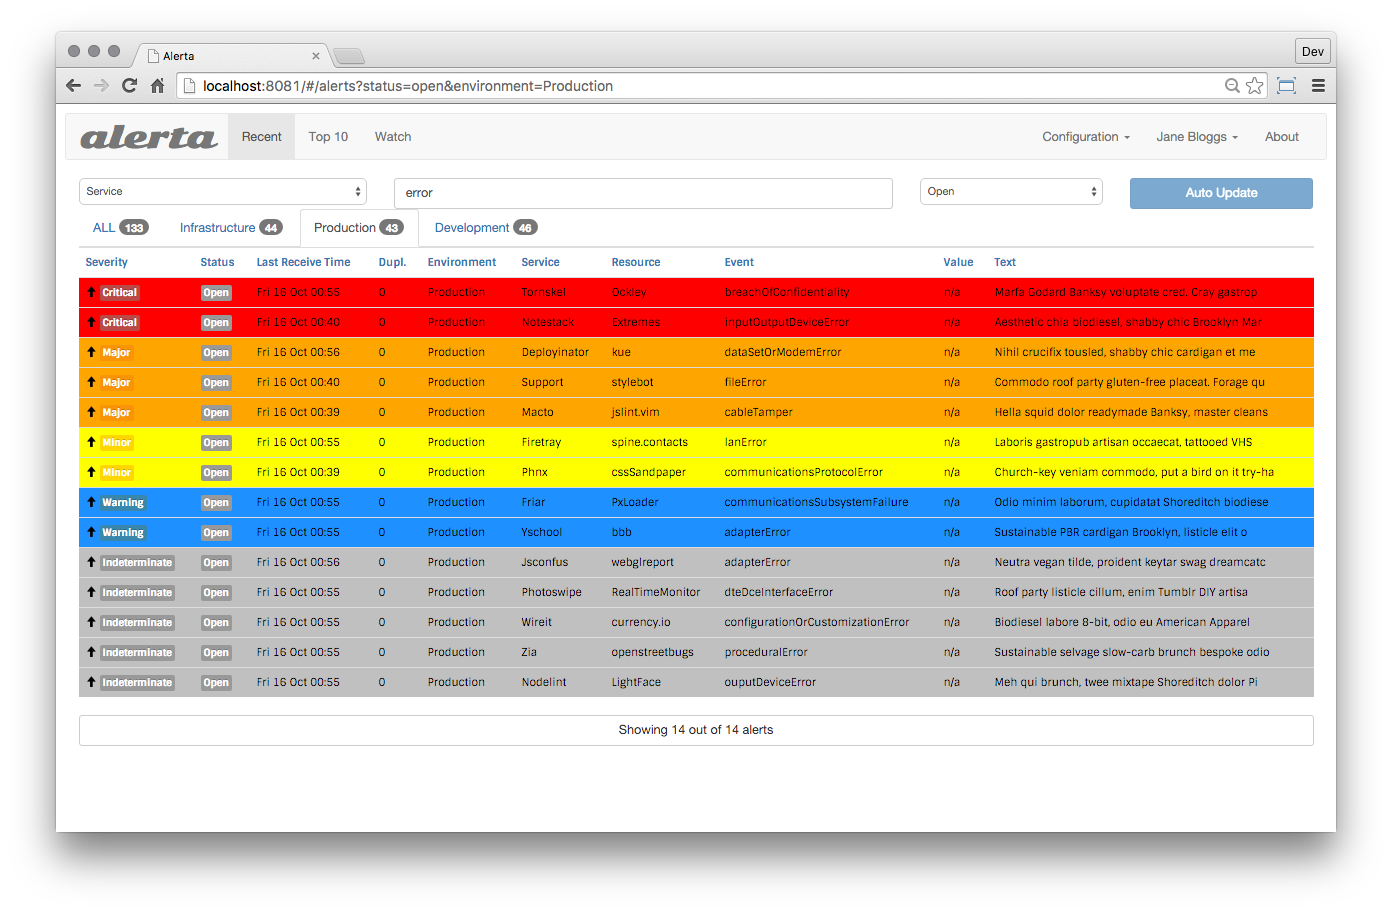
\includegraphics[width=\linewidth]{src/images/06-capitulo-6/alerta.png}
  \caption{Cliente de \gls{term:alerta} agrupando alertas por prioridades}
  \label{fig:alerta}
\end{figure}

En la \autoref{fig:alerta} se puede ver cómo se ven las alertas listadas en el
cliente de \gls{term:alerta}. La herramienta se encarga de ordenarlas por grado
de severidad, y agruparlas, de forma que no aparezcan las alertas repetidas,
sino que aparezcan una única vez, especificando la cantidad de repeticiones con
un contador.

En este capítulo hemos mostrado cómo instalar y configurar \gls{term:kapacitor}
para generar alertas. Cómo definir alertas utilizando el lenguaje
\gls{term:tick_script} y cómo resolver el problema de visualización y manejo de
alertas agregando \gls{term:alerta} a la lista de herramientas.

Con ésto hemos completado la parte práctica de nuestro trabajo. A continuación
daremos nuestras conclusiones finales de la tesis.
